% Created by tikzDevice version 0.8.1 on 2015-06-28 20:20:30
% !TEX encoding = UTF-8 Unicode
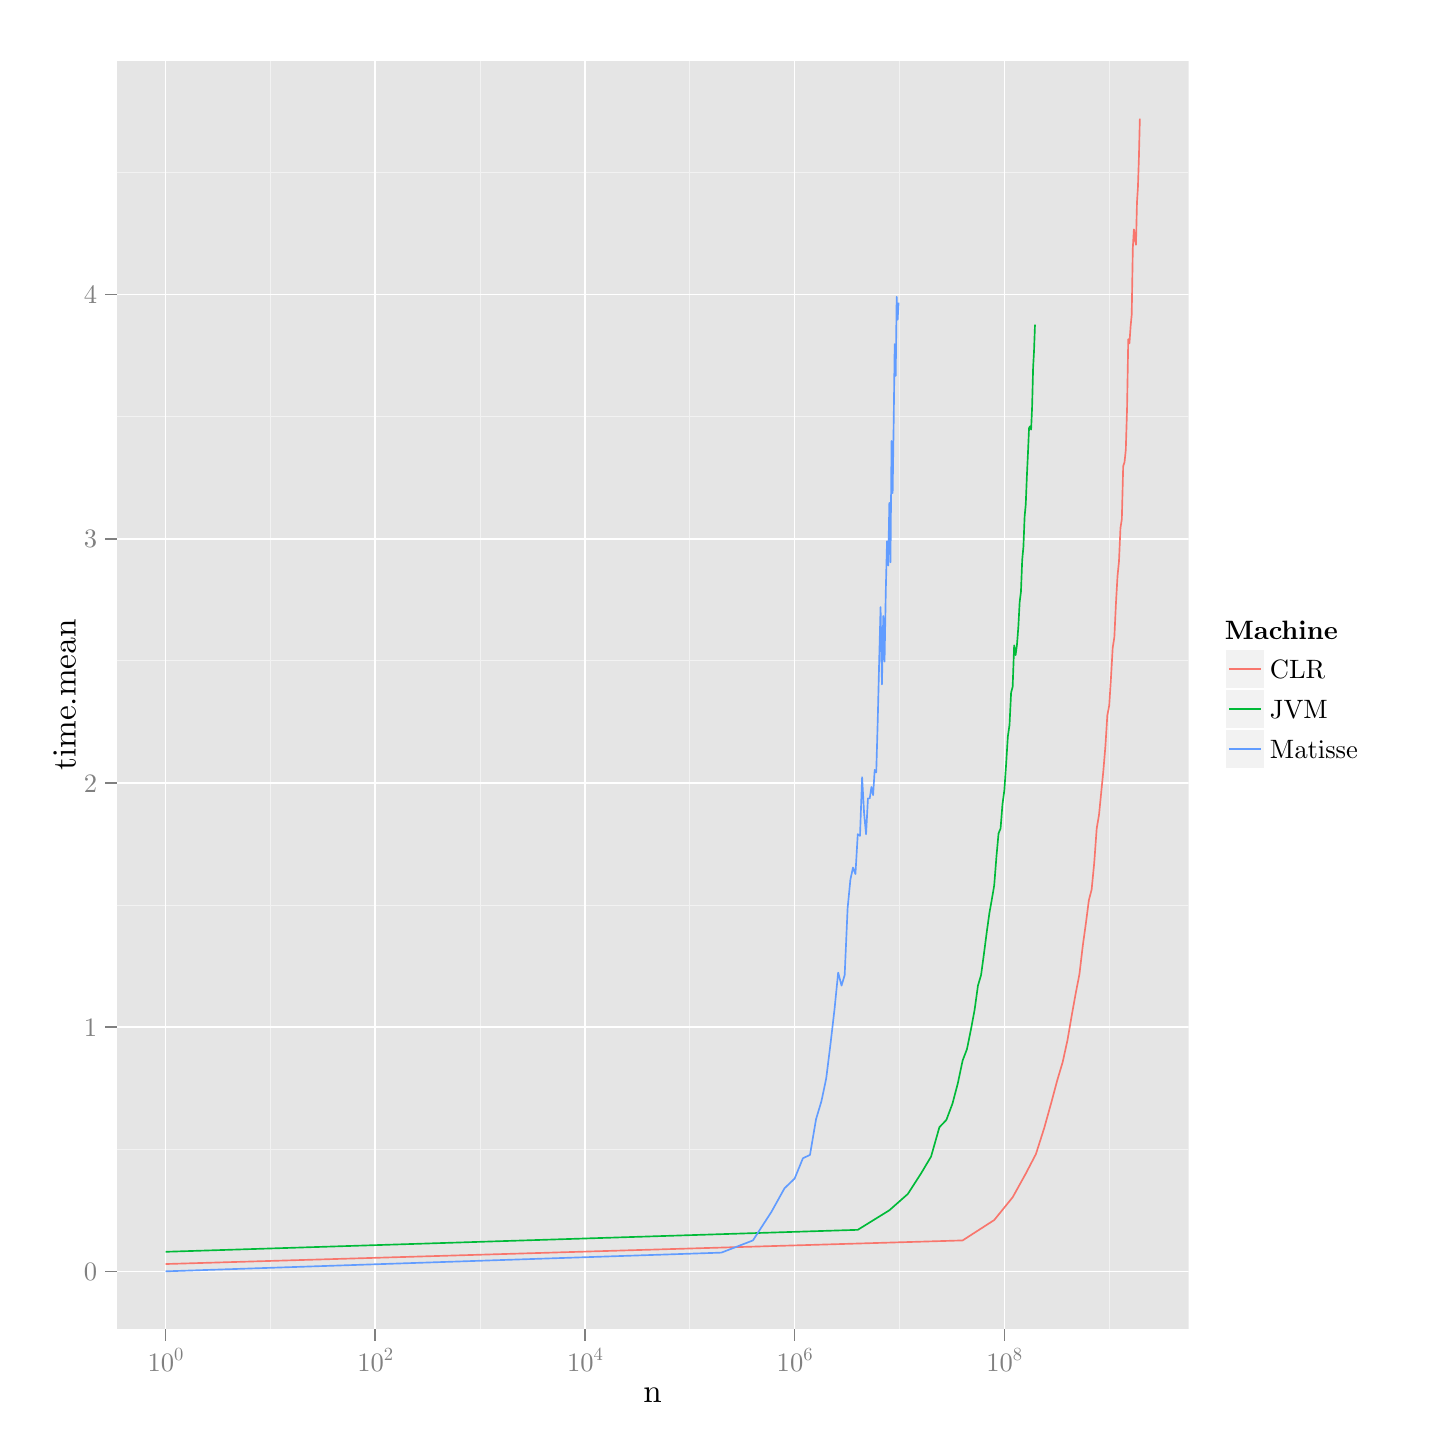
\begin{tikzpicture}[x=1pt,y=1pt]
\definecolor{fillColor}{RGB}{255,255,255}
\path[use as bounding box,fill=fillColor,fill opacity=0.00] (0,0) rectangle (505.89,505.89);
\begin{scope}
\path[clip] (  0.00,  0.00) rectangle (505.89,505.89);
\definecolor{drawColor}{RGB}{255,255,255}
\definecolor{fillColor}{RGB}{255,255,255}

\path[draw=drawColor,line width= 0.6pt,line join=round,line cap=round,fill=fillColor] (  0.00,  0.00) rectangle (505.89,505.89);
\end{scope}
\begin{scope}
\path[clip] ( 32.22, 35.66) rectangle (419.48,493.85);
\definecolor{fillColor}{gray}{0.90}

\path[fill=fillColor] ( 32.22, 35.66) rectangle (419.48,493.85);
\definecolor{drawColor}{gray}{0.95}

\path[draw=drawColor,line width= 0.3pt,line join=round] ( 32.22,100.61) --
	(419.48,100.61);

\path[draw=drawColor,line width= 0.3pt,line join=round] ( 32.22,188.86) --
	(419.48,188.86);

\path[draw=drawColor,line width= 0.3pt,line join=round] ( 32.22,277.11) --
	(419.48,277.11);

\path[draw=drawColor,line width= 0.3pt,line join=round] ( 32.22,365.36) --
	(419.48,365.36);

\path[draw=drawColor,line width= 0.3pt,line join=round] ( 32.22,453.60) --
	(419.48,453.60);

\path[draw=drawColor,line width= 0.3pt,line join=round] ( 87.71, 35.66) --
	( 87.71,493.85);

\path[draw=drawColor,line width= 0.3pt,line join=round] (163.48, 35.66) --
	(163.48,493.85);

\path[draw=drawColor,line width= 0.3pt,line join=round] (239.26, 35.66) --
	(239.26,493.85);

\path[draw=drawColor,line width= 0.3pt,line join=round] (315.03, 35.66) --
	(315.03,493.85);

\path[draw=drawColor,line width= 0.3pt,line join=round] (390.81, 35.66) --
	(390.81,493.85);
\definecolor{drawColor}{RGB}{255,255,255}

\path[draw=drawColor,line width= 0.6pt,line join=round] ( 32.22, 56.49) --
	(419.48, 56.49);

\path[draw=drawColor,line width= 0.6pt,line join=round] ( 32.22,144.73) --
	(419.48,144.73);

\path[draw=drawColor,line width= 0.6pt,line join=round] ( 32.22,232.98) --
	(419.48,232.98);

\path[draw=drawColor,line width= 0.6pt,line join=round] ( 32.22,321.23) --
	(419.48,321.23);

\path[draw=drawColor,line width= 0.6pt,line join=round] ( 32.22,409.48) --
	(419.48,409.48);

\path[draw=drawColor,line width= 0.6pt,line join=round] ( 49.82, 35.66) --
	( 49.82,493.85);

\path[draw=drawColor,line width= 0.6pt,line join=round] (125.60, 35.66) --
	(125.60,493.85);

\path[draw=drawColor,line width= 0.6pt,line join=round] (201.37, 35.66) --
	(201.37,493.85);

\path[draw=drawColor,line width= 0.6pt,line join=round] (277.14, 35.66) --
	(277.14,493.85);

\path[draw=drawColor,line width= 0.6pt,line join=round] (352.92, 35.66) --
	(352.92,493.85);
\definecolor{drawColor}{RGB}{248,118,109}

\path[draw=drawColor,line width= 0.6pt,line join=round] ( 49.82, 59.13) --
	(337.84, 67.66) --
	(349.25, 75.02) --
	(355.92, 83.25) --
	(360.65, 91.79) --
	(364.32, 98.85) --
	(367.32,108.26) --
	(369.86,117.38) --
	(372.06,125.61) --
	(373.99,132.09) --
	(375.73,140.03) --
	(377.30,149.15) --
	(378.73,157.09) --
	(380.05,163.85) --
	(381.26,174.15) --
	(382.40,182.39) --
	(383.46,190.62) --
	(384.46,194.45) --
	(385.40,204.16) --
	(386.29,216.51) --
	(387.13,221.51) --
	(387.94,229.75) --
	(388.70,237.40) --
	(389.43,246.22) --
	(390.13,257.40) --
	(390.81,260.93) --
	(391.45,270.93) --
	(392.07,281.81) --
	(392.67,285.64) --
	(393.25,297.99) --
	(393.81,307.70) --
	(394.34,312.99) --
	(394.87,325.06) --
	(395.37,328.29) --
	(395.86,347.41) --
	(396.34,348.88) --
	(396.80,353.29) --
	(397.26,368.30) --
	(397.69,393.30) --
	(398.12,391.83) --
	(398.54,398.01) --
	(398.94,402.13) --
	(399.34,426.25) --
	(399.73,433.01) --
	(400.11,429.48) --
	(400.48,427.42) --
	(400.84,442.72) --
	(401.19,448.31) --
	(401.54,458.90) --
	(401.88,473.02);
\definecolor{drawColor}{RGB}{0,186,56}

\path[draw=drawColor,line width= 0.6pt,line join=round] ( 49.82, 63.55) --
	(299.95, 71.49) --
	(311.36, 78.55) --
	(318.03, 84.43) --
	(322.77, 91.79) --
	(326.44, 97.96) --
	(329.44,108.55) --
	(331.97,111.20) --
	(334.17,117.08) --
	(336.11,124.44) --
	(337.84,132.67) --
	(339.41,136.79) --
	(340.84,143.85) --
	(342.16,150.91) --
	(343.38,159.74) --
	(344.51,163.56) --
	(345.58,171.50) --
	(346.57,179.15) --
	(347.51,185.92) --
	(348.40,190.92) --
	(349.25,195.92) --
	(350.05,206.21) --
	(350.82,214.74) --
	(351.55,216.51) --
	(352.25,225.33) --
	(352.92,230.34) --
	(353.56,239.75) --
	(354.18,249.75) --
	(354.78,253.87) --
	(355.36,265.63) --
	(355.92,267.69) --
	(356.46,282.70) --
	(356.98,279.17) --
	(357.49,282.99) --
	(357.98,289.46) --
	(358.45,298.29) --
	(358.92,302.11) --
	(359.37,313.58) --
	(359.81,318.29) --
	(360.24,329.17) --
	(360.65,333.59) --
	(361.06,343.88) --
	(361.45,352.12) --
	(361.84,361.24) --
	(362.22,361.83) --
	(362.59,360.65) --
	(362.95,368.89) --
	(363.31,383.01) --
	(363.65,389.18) --
	(363.99,398.60);
\definecolor{drawColor}{RGB}{97,156,255}

\path[draw=drawColor,line width= 0.6pt,line join=round] ( 49.82, 56.49) --
	(250.66, 63.25) --
	(262.07, 67.66) --
	(268.74, 77.96) --
	(273.47, 86.49) --
	(277.14, 90.02) --
	(280.14, 97.37) --
	(282.68, 98.55) --
	(284.88,111.49) --
	(286.82,117.97) --
	(288.55,126.20) --
	(290.12,138.85) --
	(291.55,151.21) --
	(292.87,164.44) --
	(294.09,159.74) --
	(295.22,163.56) --
	(296.28,187.68) --
	(297.28,197.98) --
	(298.22,202.39) --
	(299.11,200.04) --
	(299.95,214.45) --
	(300.76,213.86) --
	(301.52,235.04) --
	(302.25,221.80) --
	(302.95,214.45) --
	(303.63,227.39) --
	(304.27,227.39) --
	(304.89,231.51) --
	(305.49,228.57) --
	(306.07,237.69) --
	(306.63,236.81) --
	(307.17,255.63) --
	(307.69,277.11) --
	(308.19,296.52) --
	(308.69,268.58) --
	(309.16,293.29) --
	(309.63,276.81) --
	(310.08,302.40) --
	(310.52,320.35) --
	(310.94,311.52) --
	(311.36,334.17) --
	(311.77,312.70) --
	(312.16,356.53) --
	(312.55,337.70) --
	(312.93,363.30) --
	(313.30,391.54) --
	(313.66,380.06) --
	(314.01,408.60) --
	(314.36,400.36) --
	(314.70,406.54);
\end{scope}
\begin{scope}
\path[clip] (  0.00,  0.00) rectangle (505.89,505.89);
\definecolor{drawColor}{gray}{0.50}

\node[text=drawColor,anchor=base east,inner sep=0pt, outer sep=0pt, scale=  0.96] at ( 25.11, 53.18) {0};

\node[text=drawColor,anchor=base east,inner sep=0pt, outer sep=0pt, scale=  0.96] at ( 25.11,141.43) {1};

\node[text=drawColor,anchor=base east,inner sep=0pt, outer sep=0pt, scale=  0.96] at ( 25.11,229.68) {2};

\node[text=drawColor,anchor=base east,inner sep=0pt, outer sep=0pt, scale=  0.96] at ( 25.11,317.93) {3};

\node[text=drawColor,anchor=base east,inner sep=0pt, outer sep=0pt, scale=  0.96] at ( 25.11,406.17) {4};
\end{scope}
\begin{scope}
\path[clip] (  0.00,  0.00) rectangle (505.89,505.89);
\definecolor{drawColor}{gray}{0.50}

\path[draw=drawColor,line width= 0.6pt,line join=round] ( 27.95, 56.49) --
	( 32.22, 56.49);

\path[draw=drawColor,line width= 0.6pt,line join=round] ( 27.95,144.73) --
	( 32.22,144.73);

\path[draw=drawColor,line width= 0.6pt,line join=round] ( 27.95,232.98) --
	( 32.22,232.98);

\path[draw=drawColor,line width= 0.6pt,line join=round] ( 27.95,321.23) --
	( 32.22,321.23);

\path[draw=drawColor,line width= 0.6pt,line join=round] ( 27.95,409.48) --
	( 32.22,409.48);
\end{scope}
\begin{scope}
\path[clip] (  0.00,  0.00) rectangle (505.89,505.89);
\definecolor{drawColor}{gray}{0.50}

\path[draw=drawColor,line width= 0.6pt,line join=round] ( 49.82, 31.39) --
	( 49.82, 35.66);

\path[draw=drawColor,line width= 0.6pt,line join=round] (125.60, 31.39) --
	(125.60, 35.66);

\path[draw=drawColor,line width= 0.6pt,line join=round] (201.37, 31.39) --
	(201.37, 35.66);

\path[draw=drawColor,line width= 0.6pt,line join=round] (277.14, 31.39) --
	(277.14, 35.66);

\path[draw=drawColor,line width= 0.6pt,line join=round] (352.92, 31.39) --
	(352.92, 35.66);
\end{scope}
\begin{scope}
\path[clip] (  0.00,  0.00) rectangle (505.89,505.89);
\definecolor{drawColor}{gray}{0.50}

\node[text=drawColor,anchor=base west,inner sep=0pt, outer sep=0pt, scale=  0.96] at ( 43.35, 20.31) {10};

\node[text=drawColor,anchor=base west,inner sep=0pt, outer sep=0pt, scale=  0.67] at ( 52.94, 24.24) {0};

\node[text=drawColor,anchor=base west,inner sep=0pt, outer sep=0pt, scale=  0.96] at (119.12, 20.31) {10};

\node[text=drawColor,anchor=base west,inner sep=0pt, outer sep=0pt, scale=  0.67] at (128.72, 24.24) {2};

\node[text=drawColor,anchor=base west,inner sep=0pt, outer sep=0pt, scale=  0.96] at (194.89, 20.31) {10};

\node[text=drawColor,anchor=base west,inner sep=0pt, outer sep=0pt, scale=  0.67] at (204.49, 24.24) {4};

\node[text=drawColor,anchor=base west,inner sep=0pt, outer sep=0pt, scale=  0.96] at (270.67, 20.31) {10};

\node[text=drawColor,anchor=base west,inner sep=0pt, outer sep=0pt, scale=  0.67] at (280.26, 24.24) {6};

\node[text=drawColor,anchor=base west,inner sep=0pt, outer sep=0pt, scale=  0.96] at (346.44, 20.31) {10};

\node[text=drawColor,anchor=base west,inner sep=0pt, outer sep=0pt, scale=  0.67] at (356.04, 24.24) {8};
\end{scope}
\begin{scope}
\path[clip] (  0.00,  0.00) rectangle (505.89,505.89);
\definecolor{drawColor}{RGB}{0,0,0}

\node[text=drawColor,anchor=base,inner sep=0pt, outer sep=0pt, scale=  1.20] at (225.85,  9.03) {n};
\end{scope}
\begin{scope}
\path[clip] (  0.00,  0.00) rectangle (505.89,505.89);
\definecolor{drawColor}{RGB}{0,0,0}

\node[text=drawColor,rotate= 90.00,anchor=base,inner sep=0pt, outer sep=0pt, scale=  1.20] at ( 17.30,264.75) {time.mean};
\end{scope}
\begin{scope}
\path[clip] (  0.00,  0.00) rectangle (505.89,505.89);
\definecolor{fillColor}{RGB}{255,255,255}

\path[fill=fillColor] (428.35,233.68) rectangle (484.98,295.82);
\end{scope}
\begin{scope}
\path[clip] (  0.00,  0.00) rectangle (505.89,505.89);
\definecolor{drawColor}{RGB}{0,0,0}

\node[text=drawColor,anchor=base west,inner sep=0pt, outer sep=0pt, scale=  0.96] at (432.62,284.93) {\bfseries Machine};
\end{scope}
\begin{scope}
\path[clip] (  0.00,  0.00) rectangle (505.89,505.89);
\definecolor{drawColor}{RGB}{255,255,255}
\definecolor{fillColor}{gray}{0.95}

\path[draw=drawColor,line width= 0.6pt,line join=round,line cap=round,fill=fillColor] (432.62,266.86) rectangle (447.07,281.31);
\end{scope}
\begin{scope}
\path[clip] (  0.00,  0.00) rectangle (505.89,505.89);
\definecolor{drawColor}{RGB}{248,118,109}

\path[draw=drawColor,line width= 0.6pt,line join=round] (434.06,274.09) -- (445.62,274.09);
\end{scope}
\begin{scope}
\path[clip] (  0.00,  0.00) rectangle (505.89,505.89);
\definecolor{drawColor}{RGB}{255,255,255}
\definecolor{fillColor}{gray}{0.95}

\path[draw=drawColor,line width= 0.6pt,line join=round,line cap=round,fill=fillColor] (432.62,252.41) rectangle (447.07,266.86);
\end{scope}
\begin{scope}
\path[clip] (  0.00,  0.00) rectangle (505.89,505.89);
\definecolor{drawColor}{RGB}{0,186,56}

\path[draw=drawColor,line width= 0.6pt,line join=round] (434.06,259.63) -- (445.62,259.63);
\end{scope}
\begin{scope}
\path[clip] (  0.00,  0.00) rectangle (505.89,505.89);
\definecolor{drawColor}{RGB}{255,255,255}
\definecolor{fillColor}{gray}{0.95}

\path[draw=drawColor,line width= 0.6pt,line join=round,line cap=round,fill=fillColor] (432.62,237.95) rectangle (447.07,252.41);
\end{scope}
\begin{scope}
\path[clip] (  0.00,  0.00) rectangle (505.89,505.89);
\definecolor{drawColor}{RGB}{97,156,255}

\path[draw=drawColor,line width= 0.6pt,line join=round] (434.06,245.18) -- (445.62,245.18);
\end{scope}
\begin{scope}
\path[clip] (  0.00,  0.00) rectangle (505.89,505.89);
\definecolor{drawColor}{RGB}{0,0,0}

\node[text=drawColor,anchor=base west,inner sep=0pt, outer sep=0pt, scale=  0.96] at (448.88,270.78) {CLR};
\end{scope}
\begin{scope}
\path[clip] (  0.00,  0.00) rectangle (505.89,505.89);
\definecolor{drawColor}{RGB}{0,0,0}

\node[text=drawColor,anchor=base west,inner sep=0pt, outer sep=0pt, scale=  0.96] at (448.88,256.33) {JVM};
\end{scope}
\begin{scope}
\path[clip] (  0.00,  0.00) rectangle (505.89,505.89);
\definecolor{drawColor}{RGB}{0,0,0}

\node[text=drawColor,anchor=base west,inner sep=0pt, outer sep=0pt, scale=  0.96] at (448.88,241.87) {Matisse};
\end{scope}
\end{tikzpicture}
